% ------------------------------------------------------------------------------
Openquake is the core of the OpenGEM system. 

As it appears in Figure \ref{fig:oq_it}, OpenQuake is powered by a 
number of open source software projects, of which OpenSHA-lite and 
RiskLib are currently the most essential ones. 
OpenSHA-lite is a ‘light’ version of the comprehensive software for 
probabilistic seismic hazard assessment OpenSHA and whose code serves
as a basis for the hazard component of the OpenQuake engine. RiskLib 
is a global collaboration project that is aimed at common development 
of a code ‘library’ for the risk all types of natural hazards, including
an API, on wh ich ‘apps’ can be built, such as tools that support risk
mitigation/reduction. The World Bank’s GFDRR, OpenGeo, AIFDR and GEM 
jointly work on RiskLib and its code repository, currently part of 
the OpenQuake project, will be broken out soon.

Implementation of a standard format for data exchange for natural hazard
and risk,  is closely related to what is described above. The NRML 
(Natural hazards’ Risk Markup Language) format has been developed, which
is capable of encompassing a wide variety of risk and hazard data formats.
More information can be found in the detailed background documentation 
for OpenQuake.

The data services that are mentioned above are globally accessible 
read/write collaborations of core data sets that are exposed with a 
REST API. Some of the core modules of GEM will be available through 
the services and are currently being developed by GEM’s Model Facility 
development team, in collaboration with a number of IT partners and the 
scientists coordinating the modules. Examples are the development of a 
global exposure database, development of a global portal for active 
faults, global vulnerability functions and an earthquake consequences
database.

% . . . . . . . . . . . . . . . . . . . . . . . . . . . . . . . . . . . > Figure
\begin{figure}
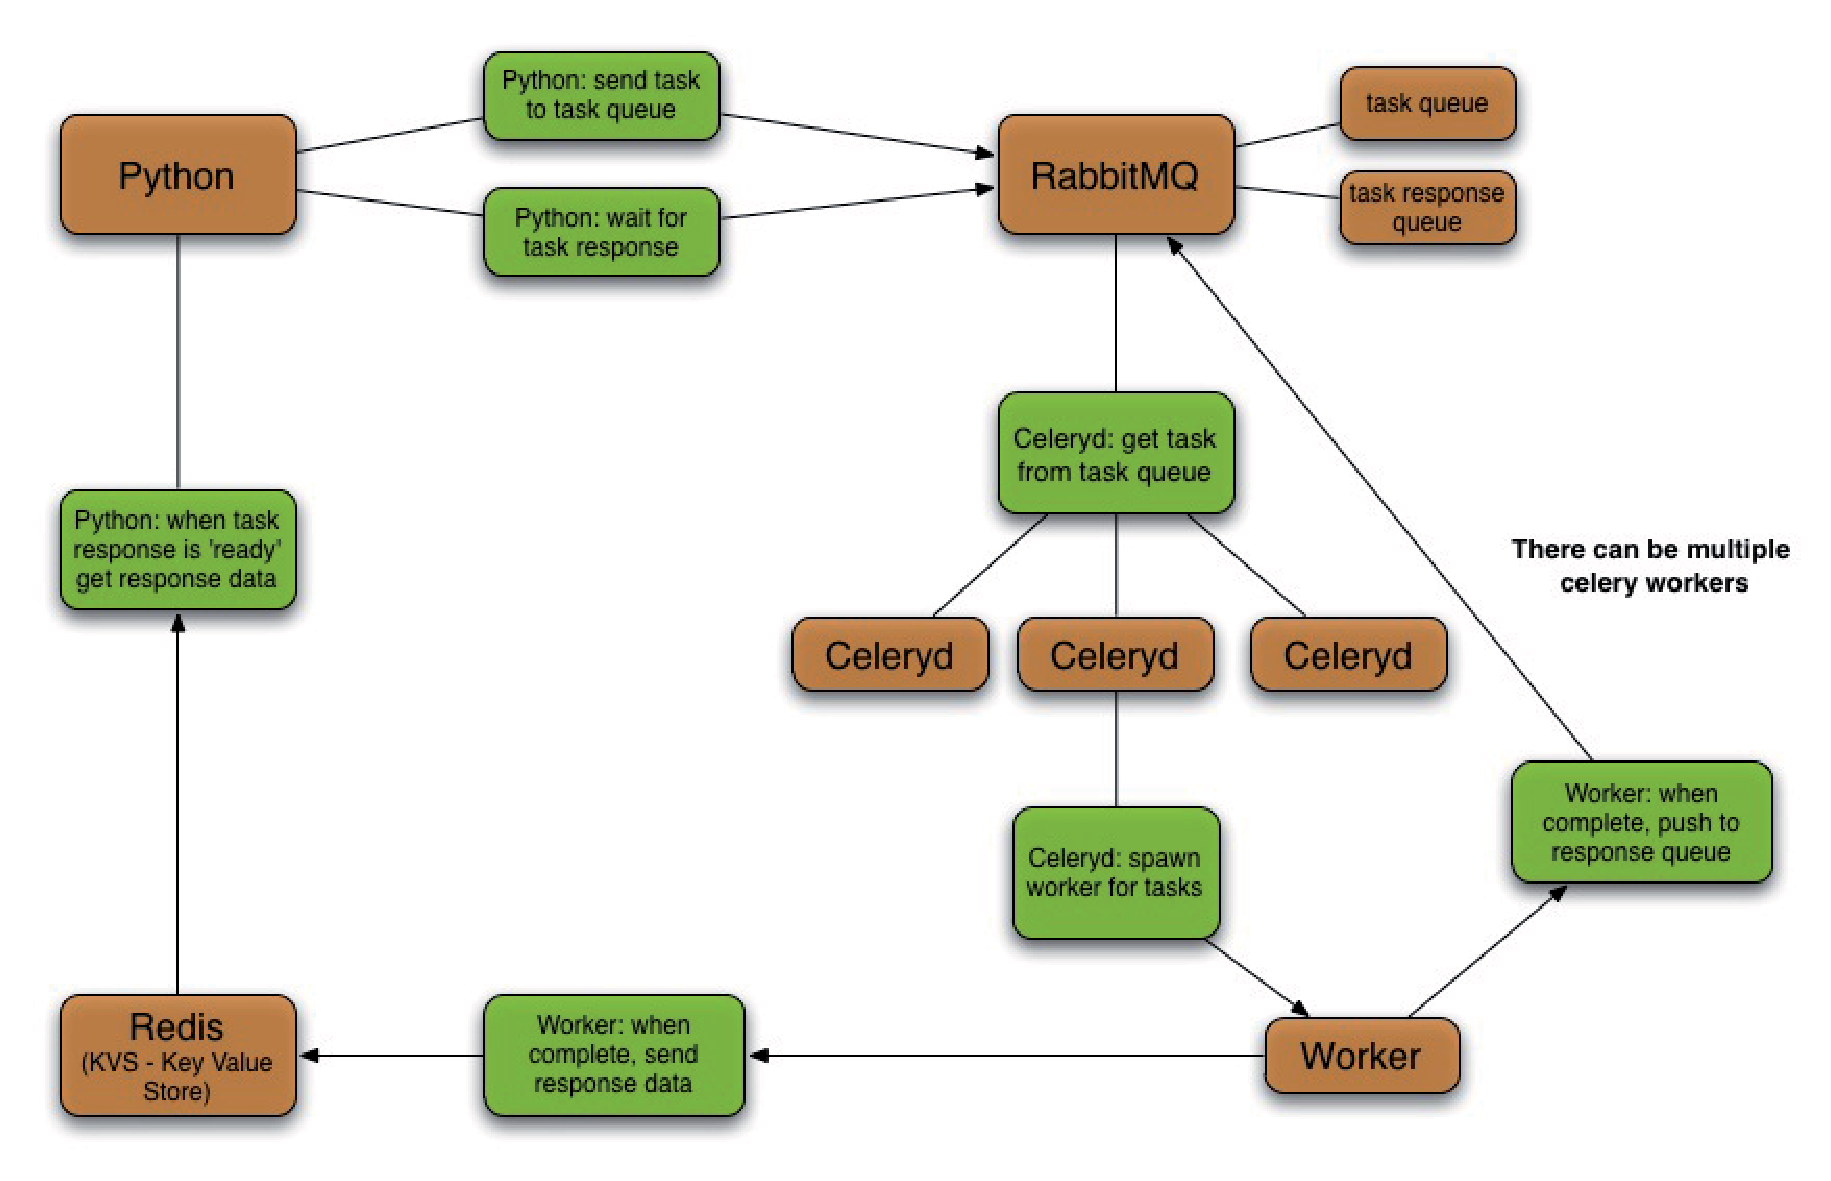
\includegraphics[width=\textwidth,angle=0]{./Figures/Part_Introduction/oq_system_architecture.eps}
\caption{Openquake system architecture.}
\label{fig:oq_it}
\end{figure}
% . . . . . . . . . . . . . . . . . . . . . . . . . . . . . . . . . . . < Figure


